\section{Ejercicio 1}\label{sec:ej1}

Tras aplicar el algoritmo de Leiden a la red de artículos de Amazon, se obtiene
una partición de 18 comunidades, con una modularidad de $0.8832$. Sin embargo,
al comparar mediante la información mutua normalizada con el \emph{ground truth},
encontramos un resultado de $0.54$, que es bastante bajo.

En la figura \ref{fig:1-circular-comp} podemos comparar los gráficos circulares
del \emph{ground truth} y de la salida del algoritmo de Leiden, usando el color
para representar la intersección entre comunidades de las dos soluciones. En la
figura \ref{fig:1-bipartite} podemos ver una comparación mediante un grafo
bipartito, donde los nodos de la izquierda representan las comunidades
\emph{ground truth} y los de la derecha las comunidades generadas por el
algoritmo de Leiden. En esta figura, tanto los colores de los nodos de la derecha
como la amplitud de las aristas representan la intersección entre comunidades de
las dos soluciones.

Vemos que la comunidad real más grande se ha dividido en muchas. También que
otras tres comunidades pequeñas quedan divididas (en dos, dos y tres
comunidades). Además, trece de las dieciocho comunidades generadas por Leiden
se corresponden con una sola comunidad real, lo que indica que no tienden
a entremezclarse comunidades reales.

\begin{figure}[!htb]
  \centering
  \begin{subfigure}{.4\textwidth}
    \centering
    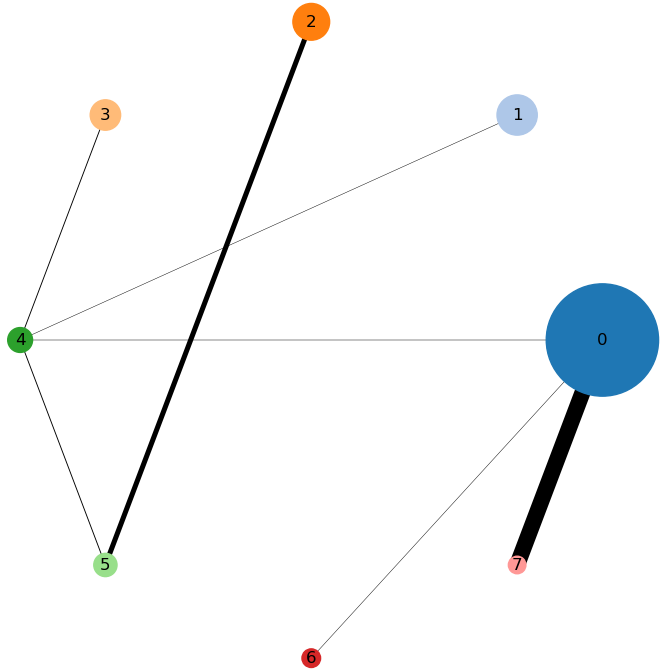
\includegraphics[width=.9\linewidth]{img/1_circular_comp_1}
    \caption{Gráfico circular de las comunidades \emph{ground truth}. }
    \label{fig:1-circular-comp-1}
  \end{subfigure}%
  \hfill
  \begin{subfigure}{.4\textwidth}
    \centering
    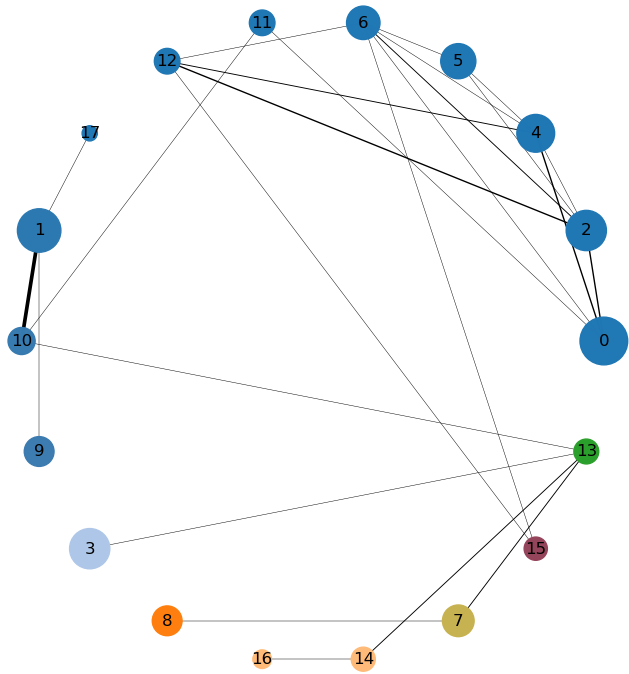
\includegraphics[width=.9\linewidth]{img/1_circular_comp_2}
    \caption{Gráfico circular de las comunidades generadas por el algoritmo de Leiden. }
    \label{fig:1-circular-comp-2}
  \end{subfigure}
  \caption{Comparación de gráficos circulares entre el \emph{ground truth} y el
    algoritmo de Leiden. Los colores de las comunidades en el gráfico de la
    derecha son una media de los del gráfico de la izquierda, en función del
    tamaño de la intersección con la comunidad correspondiente.}
  \label{fig:1-circular-comp}
\end{figure}

\begin{figure}[!htb]
  \centering
  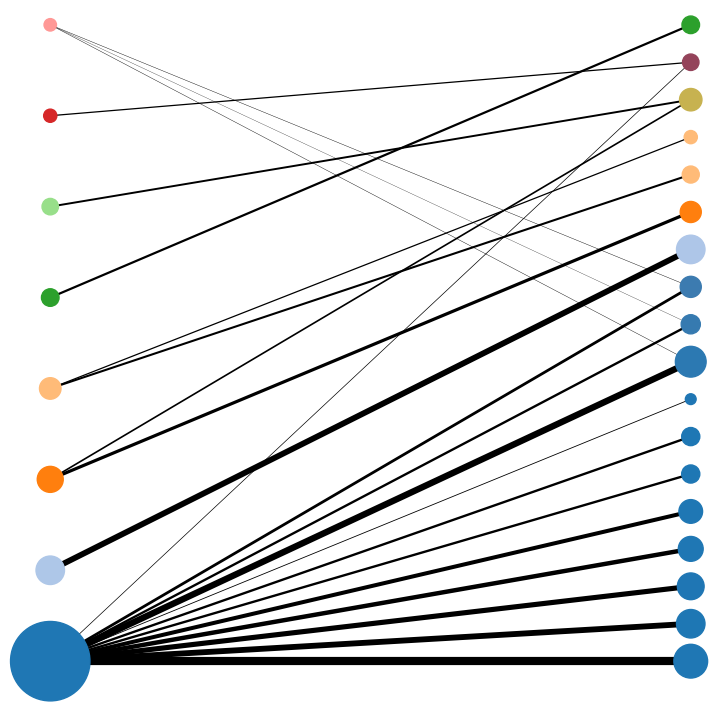
\includegraphics[width=.7\linewidth]{img/1_bipartite_comp}
  \caption{Comparación de comunidades mediante un grafo bipartito. A la
    izquierda vemos las comunidades \emph{ground truth}, y a la derecha las
    generadas por el algoritmo de Leiden.  Los colores de las comunidades en el
    gráfico de la derecha son una media de los del gráfico de la izquierda, en
    función del tamaño de la intersección con la comunidad correspondiente. La
    amplitud de las aristas muestra el número de nodos en común de las
    comunidades que conectan.}
  \label{fig:1-bipartite}
\end{figure}



Todo parece indicar un problema de resolución, como hemos visto en clase.
Recordemos que la fórmula de la modularidad se puede escribir como:
$$
\sum_{i=1}^C e_{ii} - a_i^2,
$$
donde
\begin{itemize}
  \item $e_{ij}$ es la fracción de aristas con un vértice en la comunidad $i$ y
    el otro en la $j$.
  \item $a_i$ es la fracción de aristas con algún vértice en la comunidad $i$.
\end{itemize}

Si nos fijamos, el primer término es $\sum_i e_{ii} = 1 - \sum_{i\neq j}
e_{ij}$, es decir, que para maximizar el primer término buscamos minimizar la
fracción de aristas entre comunidades. Es claro que para ello nos conviene
tener un número reducido de comunidades. En el caso extremo, si solo hubiese una
comunidad obtendríamos el valor perfecto $1$. Respecto al segundo término, se
puede descomponer como:
$$
\sum_{i=1}^C a_i^2 =
\frac{1}{(2m)^2} \sum_{i=1}^C \left( \sum_{n \in c_i} \delta(n)^2 + \sum_{n_1, n_2 \in c_i, n_1 \neq n_2} \delta(n_1) \delta(n_2) \right) 
.$$
La suma de los cuadrados es imposible de evitar, y el otro término depende de
los grados de nodos en la misma comunidad. Si los grados son bajos, se
considera que es poco probable que los nodos se crucen entre sí, y por lo tanto
una conexión entre ellos es significativa. Por lo tanto, se buscan comunidades
con pocos nodos y cuyos grados sean pequeños. En el caso extremo, si cada nodo
formase una comunidad, este término se minimizaría. Es fácil ver entonces que
esta parte de la métrica busca un mayor número de comunidades.

Este \emph{trade-off} se suele modular con un parámetro positivo $\gamma > 0$,
de la siguiente forma:
$$
\sum_{i=1}^C e_{ii} - \gamma a_i^2
.$$
Cuando $\gamma$ es grande, el algoritmo tiende a dividir comunidades grandes, y
en caso contrario a juntar comunidades pequeñas.

Con esta consideración, podemos probar a ejecutar el algoritmo de Leiden con
con diferentes valores de $\gamma$. Como la implementación no lo permite,
recurro en esta parte al algoritmo menos avanzado de Louvain. En la figura
\ref{fig:1-resolution-vs-nmi} podemos ver la información mutua normalizada con
el \emph{ground truth} en función del parámetro $\gamma$. Vemos que el valor
máximo se alcanza en $\gamma = 0.06$, con un valor ligeramente
superior a $0.7$. En la figura \ref{fig:1-best_res_bipartite} podemos ver una
comparación de las comunidades obtenidas con este valor de $\gamma$. En este caso
la comunidad grande se divide en solo tres comunidades, lo cual es una
gran mejora, pero sigue sin llegar a juntarse en una. Además, las comunidades
reales más pequeñas las junta con esas tres que corresponden a la más grande.
Finalmente, vemos que dos parejas de comunidades reales medianas quedan juntadas.

Observamos que hemos pasado de un extremo a otro salvo con la comunidad más
grande. Con una resolución alta, el algoritmo separaba las comunidades
demasiado, y con una resolución baja, tiende a juntarlas demasiado. Por lo
tanto, no parece que podamos recuperar la estructura original mediante estos
algoritmos, ni siquiera tratando de seleccionar la resolución correcta. Entre
los motivos posibles, destaco tres. El primero es la posible limitación del
algoritmo voraz. El segundo es que la topología de la red podría no reflejar del todo
correctamente las comunidades buscadas. Al fin y al cabo, las aristas representan
alta frecuencia de compra de ambos artículos juntos, pero no necesariamente
significa que los artículos sean de la misma categoría. El tercer motivo es que
puede ocurrir que distintas partes de la estructura de la red requieran distintas
resoluciones, pero esto no se puede saber a priori sin el \emph{ground truth}.
Este problema con algunos métodos multi-resolución ya fue evaluado por
\citeauthor{lancichinetti2011Limitsmodularity}
\cite{lancichinetti2011Limitsmodularity}: \emph{"We show that multiresolution
modularity suffers from two opposite coexisting problems: the tendency to merge
small subgraphs, which dominates when the resolution is low; the tendency to
split large subgraphs, which dominates when the resolution is high"}.

\begin{figure}[!htb]
  \centering
  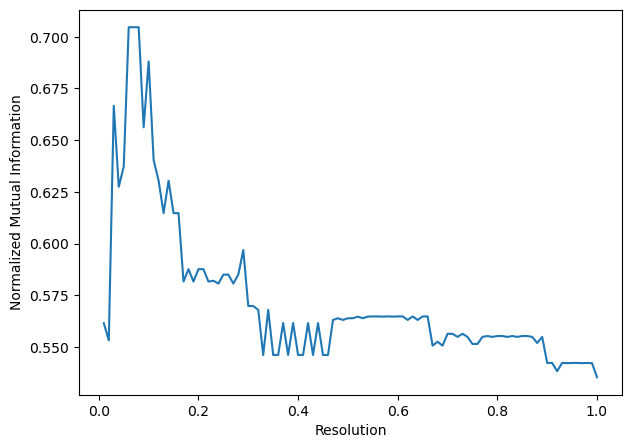
\includegraphics[width=.7\linewidth]{img/1_resolution_vs_nmi}
  \caption{Comparación de la información mutua normalizada con el \emph{ground}
    \emph{truth} en función del parámetro $\gamma$ del algoritmo de Louvain.}
  \label{fig:1-resolution-vs-nmi}
\end{figure}

\begin{figure}[!htb]
  \centering
  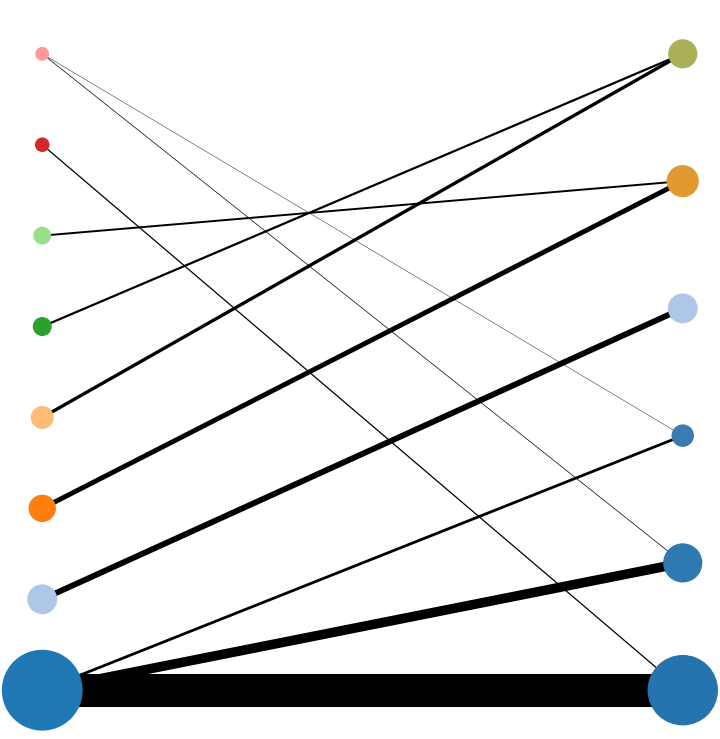
\includegraphics[width=.7\linewidth]{img/1_best_res_bipartite_comp}
  \caption{Comparación de comunidades mediante un grafo bipartito. A la
    izquierda vemos las comunidades \emph{ground truth}, y a la derecha las
    generadas por el algoritmo de Lovain con \(\gamma=0.06\).  Los colores de
    las comunidades en el gráfico de la derecha son una media de los del
    gráfico de la izquierda, en función del tamaño de la intersección con la
    comunidad correspondiente. La amplitud de las aristas muestra
    el número de nodos en común de las comunidades que conectan.}
  \label{fig:1-best_res_bipartite}
\end{figure}


